\documentclass{ujarticle}
\usepackage{robomech2022}
\usepackage[dvipdfmx]{graphicx}
\usepackage{url}
\usepackage{caption}
\captionsetup[table]{justification=centering}
\captionsetup[figure]{justification=centering}
\usepackage[subrefformat=parens]{subcaption}
\captionsetup{compatibility=false}


\begin{document}
\makeatletter
\title{視覚と行動のend-to-end学習による経路追従行動の模倣}
{―データセットを収集してオフラインで訓練する手法の検討―}
{A proposal for imitation method of path-tracking behavior by end-to-end\\ learning of vision and action}
{-Validation of a method to collect and train dataset offline-}

\author{
\begin{tabular}{lll}
 \hspace{1zw}○学\hspace{1zw}髙橋祐樹(千葉工大) & \hspace{1zw} \hspace{2zw}白須和暉(千葉工大) & \hspace{-6.5zw} 学\hspace{1zw}藤原柾(千葉工大) \\
 \hspace{2zw}正\hspace{1zw}上田隆一(千葉工大) & \hspace{1zw} 正\hspace{1zw}林原靖男(千葉工大)\\
 % ※協賛・後援団体の会員資格で発表される場合は「正・学」は不要です。
 &\\
 \multicolumn{2}{l}{\small Yuuki TAKAHASHI, Chiba Institute of Technology, s19c1068aq@s.chibakoudai.jp}\\
 \multicolumn{2}{l}{\small Kazuki SHIRASU, Masaki FUJIWARA, }\\
 \multicolumn{2}{l}{\small Ryuichi UEDA and Yasuo HYASHIBARA, Chiba Institute of Technology}\\
\end{tabular}
}
\makeatother

\abstract{ \small 
In this paper, we propose a method of training a robot by collecting data on and near a target path, based on a conventional method of imitation learning. In the proposed method, the robot is placed on and around the target path and data is collected. Then, the robot is trained off-line using the collected data. After learning, the robot runs according to the output of the trainer using camera images as input. This is performed on a simulator, and the effectiveness of the proposed method is verified through experiments. As a result, it is confirmed that the proposed method can run around the path.
}

\date{} % 日付を出力しない
\keywords{End-to-End Learning, Navigation, Offline}

\maketitle
\thispagestyle{empty}
\pagestyle{empty}

\small
\section{緒言}%===========================
本研究グループでは, end-to-end学習により, 視覚に基づく経路追従行動をオンラインで生成する手法の提案を行い, その有効性を実験により検証してきた\cite{si2020-okada}\cite{si2021-okada}. 視覚を入力として, end-to-end学習により経路追従行動を模倣する手法はいくつか提案されている. 例えば, Bojarskiらは, 人が操作するステアリングの角度をend-to-end学習することで経路追従する手法を提案した\cite{bojarski}. Jing Biらは, 歩行者が多い環境における経路追従行動の模倣に取り組んでいる\cite{pedestrian}. それに対して, 本研究グループでは, 図1に示すように, 測域センサなどを入力として自己位置推定を行い生成した行動を, カメラ画像を入力とする行動に模倣する手法を提案している. 他の手法が人の操作模倣しているのに対して, 提案手法は自動制御器の出力を模倣する点に特徴がある. \par しかし, 提案手法(以後, オンライン手法と呼ぶ)では, データ収集及び学習を行うために, ロボットを経路に沿って走行させ続けることが必要である. そのため, 経路追従の成功率を上げるためにはロボットを長時間走行させることが必要で, それが問題となっていた. \par 本稿では, 事前に収集した画像と行動を用いて, 経路追従行動をオフラインで学習する手法(以後, オフライン手法と呼ぶ)に関して検討する. これにより, オンライン手法で問題となっていた学習時間の短縮を目指す. なお,オフラインで模倣学習することは,他の研究でも行われていることであるが,そのデータを自動で収集することに本手法の特徴がある. また,本稿では,実ロボットでのデータ収集を念頭において,どの程度の経路周辺の視覚情報が必要であるかを,シミュレータを用いた実験により明らかにすることも目的とする.これにより,実ロボットを用いた学習に要する時間を短縮することを意図している.
% また, 清岡ら\cite{si2021-kiyooka}により, 経路から離れた状態も訓練データに加えた方が, 経路から離れても再び経路に戻る可能性が高いことが示されている.

% \begin{figure}[b]
%   \centering
%   \begin{minipage}[b]{0.45\linewidth}
%     \centering
%     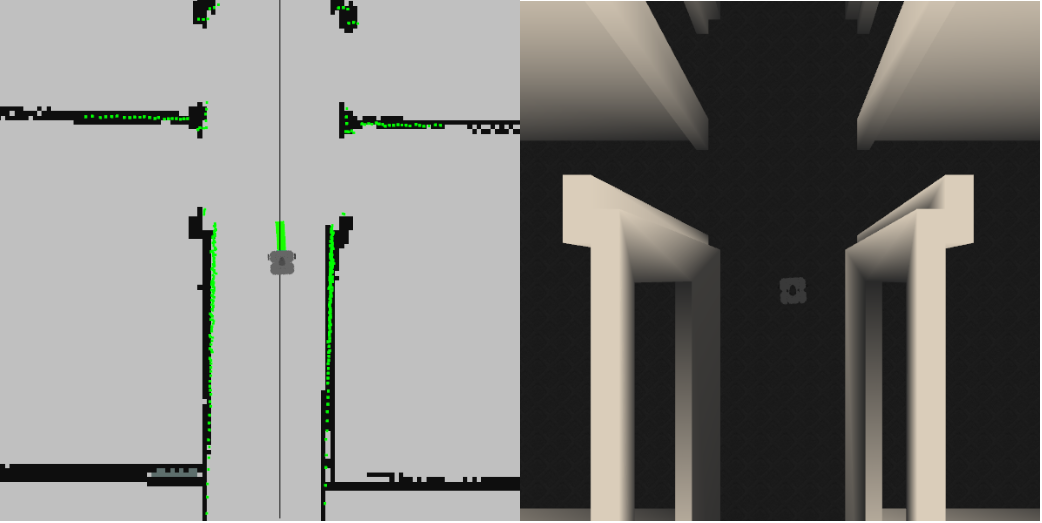
\includegraphics[width=80mm]{img/navigation.png}
%     \caption*{(a) ORNE-α}
%   \end{minipage} 
%   \hspace{0.03\columnwidth}
%   \begin{minipage}[b]{0.45\linewidth}
%     \centering
%     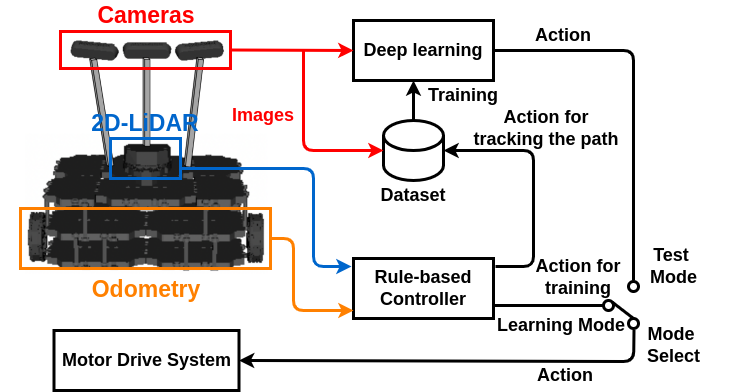
\includegraphics[height=34mm]{img/si2020-okada.png}
%     \caption*{(b) ORNE-box}
%   \end{minipage}
%   \caption{ORNE-Series}
%   \label{fig:orne-series}%\vspace*{-2mm}
% \end{figure}

\begin{figure}[h]
	\centering
	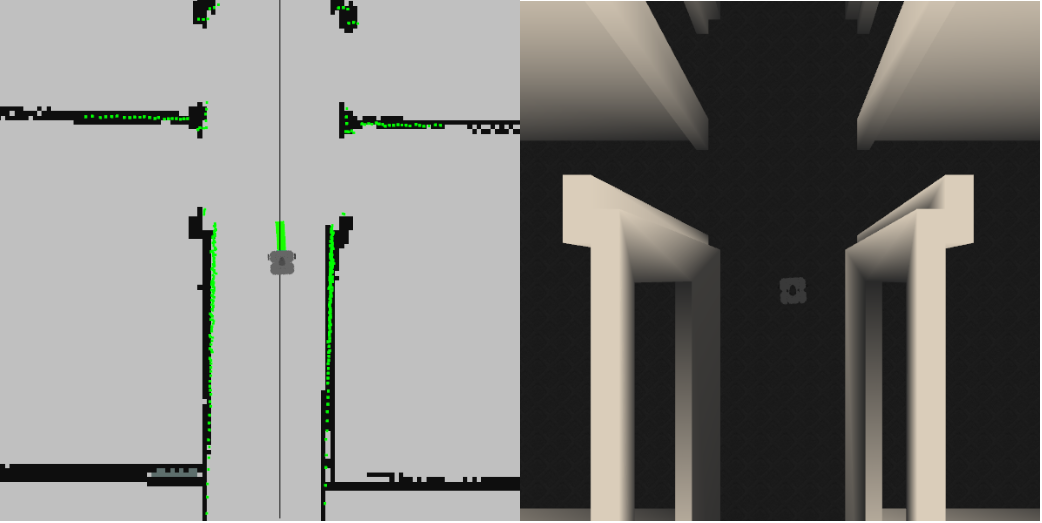
\includegraphics[width=0.37\textwidth]{img/navigation.png}
	\caption{Moving with map-based navigation}
	\label{Fig:navigation}
\end{figure}

\section{オンライン手法}%===========================
従来から提案するオンライン手法に関して述べる. オンライン手法では, 地図を用いたルールベース制御器の出力を模倣して, 経路追従行動を獲得する. 図\ref{Fig:si2020-okada}, \ref{Fig:si2020-okada-test}にシステムの概要を示すが, 手法は学習とテストの2つのフェーズで構成される. 学習フェーズでは, 測域センサとオドメトリを入力として, ROSのnavigation\cite{navigation}により, 目標角速度を求めて, ロボットを経路追従させる. 同時に64×48にリサイズした3つのカメラ画像(RGB画像)を入力, 目標角速度を出力とするデータを, データセットに加える. そのデータをランダムにピックアップしてリアルタイムに学習する. 左右のカメラ画像に対する目標角速度には, それぞれ経路に戻るようなオフセットを加える. 訓練後は, 図\ref{Fig:si2020-okada-test}のようにカメラ画像を入力とした学習器の出力を目標角速度としてロボットを制御する. テストフェーズでは3台のカメラのうち, 中央のカメラのみ使用する. なお, 目標の並進速度は0.2[m/s]で一定の速度をロボットに与える. \par オンライン手法のネットワークの構造を図\ref{Fig:cnn}に示す. 入力層1, 畳み込み層3, 全結合層2, 出力層1の全7層から構成される.  

\begin{figure}[h]
	\centering
	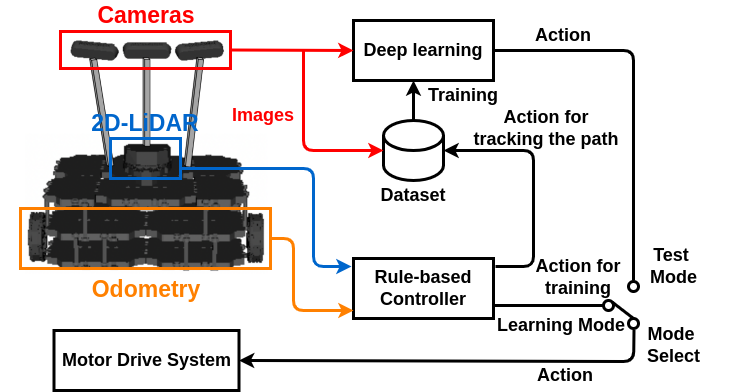
\includegraphics[width=0.5\textwidth]{img/si2020-okada.png}
	\caption{Learning phase}
	\label{Fig:si2020-okada}
\end{figure}

\begin{figure}[h]
	\centering
	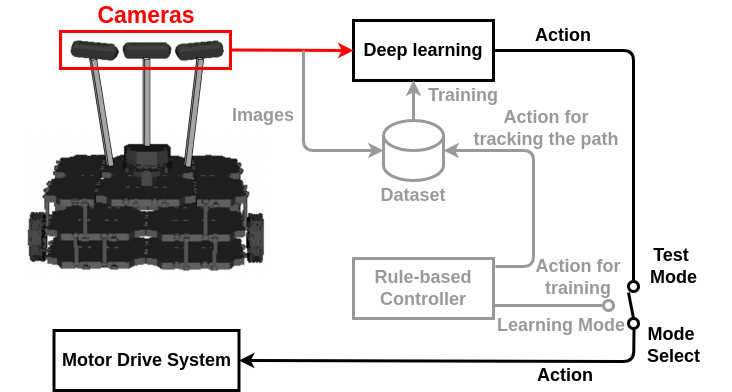
\includegraphics[width=0.5\textwidth]{img/si2020-okada-test.png}
	\caption{Test phase}
	\label{Fig:si2020-okada-test}
\end{figure}

\begin{figure}[h]
	\centering
	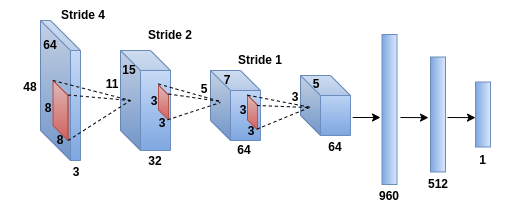
\includegraphics[width=0.45\textwidth]{img/cnn.png}
	\caption{Structure of network}
	\label{Fig:cnn}
\end{figure}

\newpage
\section{オフライン手法}%===========================
本研究で検証するオフライン手法に関して述べる. オンライン手法と比べて, オフライン手法は画像と角速度のデータを事前に収集して, オフラインで学習するところが異なる. 図\ref{Fig:collect}にシミュレータを用いたデータの収集方法を示す. 目標経路(赤線)から一定距離の位置にロボットを配置して, さらに目標経路の方向を基準にして, ヨー方向に一定量回転させる. その状態で中央のカメラの画像と,目標角速度を収集してデータセットに加える.本手法でデータを収集するためには,非常に多くのロボットの置き直しをしなければならないため,実ロボットにそのまま応用するのは難しい手法といえる.ただし,1台のロボットに複数のカメラを搭載して, 複数の視点の画像を得ることで同様にデータを収集できるため,実ロボットへの応用は可能であると考える.このように収集したデータセットを用いてオフラインで学習を行う.

\begin{figure}[h]
		\centering
		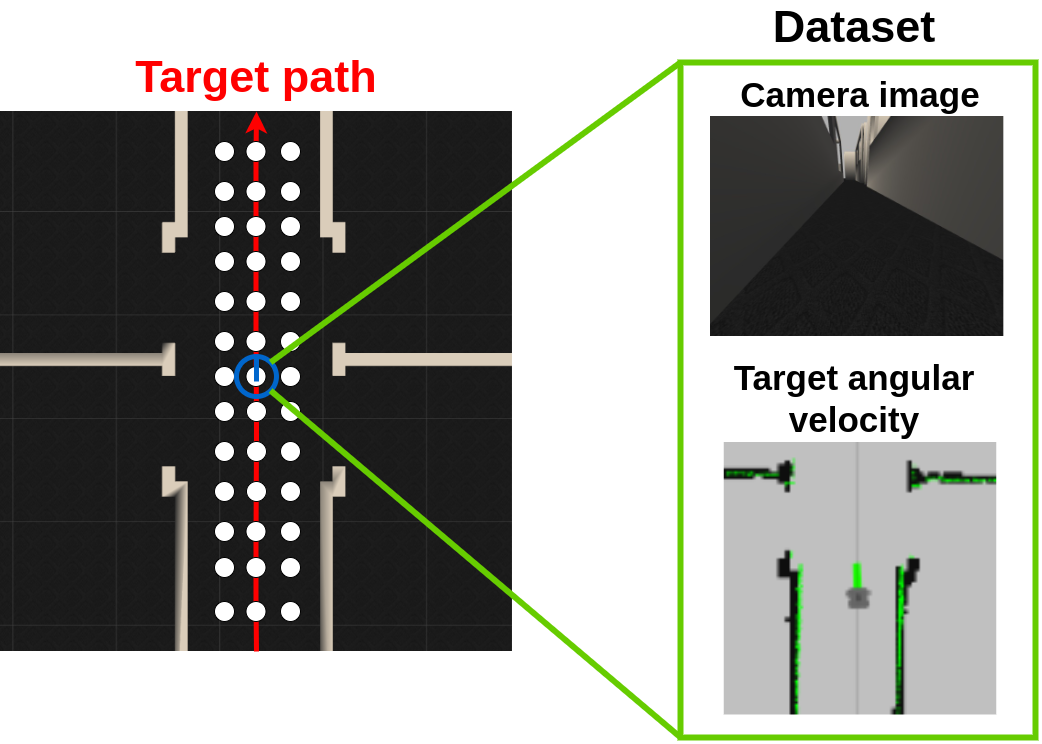
\includegraphics[width=0.45\textwidth]{img/proposed.png}
		\caption{Method of collecting data around the target path}
		\label{Fig:collect}
\end{figure}

\newpage
\section{シミュレータを用いた実験}%=========================== 
オフライン手法で経路追従できるかを実験により検証する.また,どの程度の画像情報と目標角速度のデータがあれば,経路追従できるかを明らかにする.
\subsection{実験装置}シミュレータにはGazebo\cite{gazebo}, 環境にはWillow Garage\cite{willow}を用いて, 図\ref{Fig:willow}に示す赤線を目標経路として実験を行う. また, ロボットモデルにはTurtlebo3 Waffle Pi\cite{turtlebot3}にカメラを1つ搭載したモデルを用いた. これらを実験に用いたソフトウェアに関しては以下で公開している. \par \url{https://github.com/YuukiTakahashi4690/nav_cloning}

\begin{figure}[h]
		\centering
		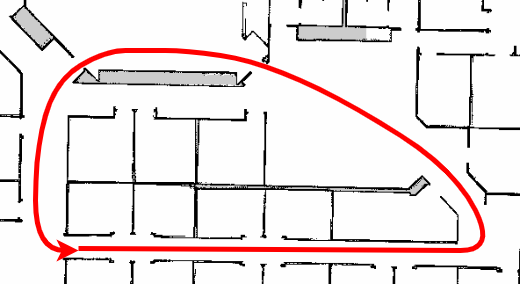
\includegraphics[width=0.4\textwidth]{img/willow-path.png}
		\caption{Course to collect data}
		\label{Fig:willow}
\end{figure}

\subsection{実験方法}
以下に実験方法を示す. 
\begin{description}
		\item[(1)データ収集フェーズ] 
		
		図\ref{Fig:collect-data}にデータの収集方法を示す. 実験1では, 赤線の目標経路上のみにロボットを配置する. 実験2では, 目標経路上には配置せずに, 経路から平行に±0.1[m]離れた位置に配置する. 実験3と実験4では, 目標経路上と経路から平行に±0.1[m]離れた位置にロボットを配置する. 実験5と実験6では, 目標経路上と経路から平行に±0.2[m]離れた位置にロボットを配置する. 実験7では, 目標経路上と経路から平行に±0.3[m]離れた位置にロボットを配置する. また, 実験1から実験7のロボットの進行方向の配置間隔は0.1[m]とする. そして, その位置ごとに目標経路の方向を基準として, ヨー方向に±5度回転させて, カメラ画像と目標角速度を収集する. ただし, 実験4と実験6のみヨー方向の回転を行わない. 
		\item[(2)学習フェーズ] 
		
		オフライン手法では, オンラインで学習を行うため, ナビゲーションなどにもコンピュータのリソースが必要であるため, バッチ数8のミニバッチ学習を採用していた. しかし, 本手法はオフラインで学習を行うため, バッチ学習を採用している. 学習ステップ数に関しては, 実験1~7は4000stepとした. なお, 4000stepはオンライン手法において, シミュレータでの実験に用いてきたステップ数である. 
		\item[(3)テストフェーズ] 
		
		学習済みモデルを用いてロボットを走行させて図\ref{Fig:willow}に示した目標経路を追従できるかを検証する. 経路を1周できた場合を成功とし, 壁に衝突したり, 目標経路から10[m]以上離れたりした場合を失敗とした.
\end{description}
上記の(2)学習フェーズと(3)テストフェーズを10回行い,経路追従の成功率を得る.

\begin{figure}[h]
		\centering
		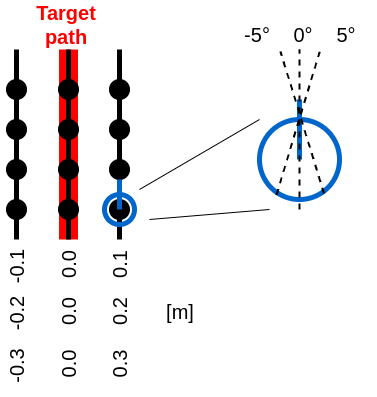
\includegraphics[width=0.45\textwidth]{img/collect2.png}
		\caption{Method of collecting data around the target route}
		\label{Fig:collect-data}
\end{figure}

\newpage
\subsection{実験結果と考察}実験結果を表\ref{tb:result}に示す. 実験1では, 角を曲がりきれずにコースアウトすることがほとんどであった. これは, 直進時の行動を学習する割合が実験2から実験4と比べて多く, 左折するデータが少ないためだと考えられる. 実験2では, 経路上のデータのみがないため, 直進時にふらつきながら走行する様子が多く見られた. 実験4は, 実験3の半分のステップ数でも成功回数があまり変わらなかった. ここで, 学習時のlossの一例を図\ref{Fig:loss}に示す. 図から実験1は, オーバフィッティングしていると考えられる. また, 実験2から実験4は学習が収束している様子が確認できる. これらのことから, 学習時に経路上及びその周辺のデータを用いる方が, 経路追従できる可能性が高いと考えられる. また, 学習時に経路上のデータを用いなくても, 概ね成功回数は変わらないことも確認できた. 因みに, 従来手法が訓練に最低40分程度必要であったのに対して, 実験3は訓練時間が4分程度であるため, 大幅に時間を短縮できることを確認した. 

\begin{table}[h]
		\caption{Number of successes in the experiments}
		\centering
		\scalebox{1.0}{
		\begin{tabular}{|c|c|} \hline
			Experiments & Number of successes \\ \hline
			Exp.1 & 0/10 \\ \hline
			Exp.2 & 8/10 \\ \hline
			Exp.3 & 9/10 \\ \hline
			Exp.4 & 0/10 \\ \hline
			Exp.5 & 10/10 \\ \hline
			Exp.6 & / \\ \hline
			Exp.7 & / \\ \hline
		\end{tabular}
		}
		\label{tb:result}
	\end{table}

\begin{figure}[h]
		\centering
		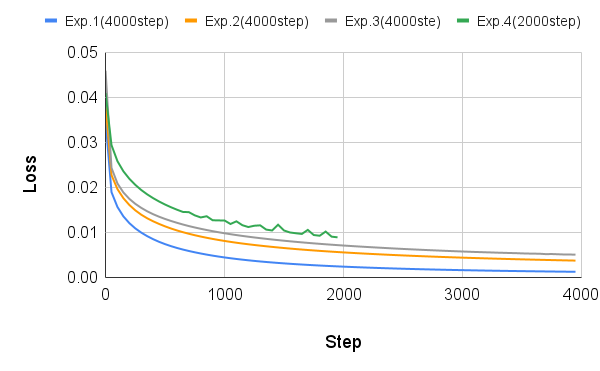
\includegraphics[width=0.5\textwidth]{img/loss_compe_fix.png}
		\caption{Loss value in the experiments}
		\label{Fig:loss}
\end{figure}

\section{結言}%===========================
本稿では, 事前に収集した画像と行動を用いて, end-to-end学習により経路追従行動をオフラインで模倣学習する手法に関して検討した. 実験により, オンライン手法で問題となっていた学習時間を大幅に短縮できることを確認した. また, 実ロボットでのデータ収集を念頭において, 必要となる経路周辺の視覚情報と目標角速度の組み合わせも, ある程度明らかにした.


\footnotesize
\begin{thebibliography}{99}

\bibitem{si2020-okada}
岡田 眞也, 清岡 優祐, 上田 隆一, 林原 靖男: ``視覚と行動のend-to-end学習により経路追従行動をオンラインで模倣する手法の提案'', \textit{計測自動制御学会 SI 部門講演会 SICE-SI2021 予稿集}, pp.1147-1152, 2020.

\bibitem{si2021-okada}
岡田 眞也, 清岡 優祐, 春山 健太, 上田 隆一, 林原 靖男: ``視覚と行動のend-to-end学習により経路追従行動をオンラインで模倣する手法の提案-“経路追従行動の修正のためにデータセットを動的に追加する手法の検討'', \textit{計測自動制御学会 SI 部門講演会 SICE-SI2021 予稿集}, pp.1066-1070, 2021.	

\bibitem{bojarski}
Bojarsi, Mariusz, et al.:``End to End Learning for Self-Driving Cars.'', arXiv: 1604.07316, 2016

\bibitem{pedestrian}
Jing Bi, Tianyou Xiao, Qiuyue Sun, Chenliang Xu. ``Navigation by Imitation in a Pedestrian-Rich Environment'', 	arXiv:1811.00506, 2018

% \bibitem{si2021-kiyooka}
% 清岡 優祐, 岡田 眞也, 岩井 一輝, 上田 隆一, 林原 靖男: ``視覚と行動のend-to-end学習により経路追従行動をオンラインで模倣する手法の提案''-データセットと生成された経路追従行動の解析'', \textit{計測自動制御学会 SI 部門講演会 SICE-SI2021 予稿集}, pp.1072-1075, 2021.

\bibitem{navigation}
ros-planning, navigation リポジトリ\\
\url{https://github.com/ros-planning/navigation}\\
(最終閲覧日 \today)

\bibitem{gazebo}
gazebo リポジトリ\\
\url{http://gazebosim.org/}\\
(最終閲覧日 \today)

\bibitem{willow}
Koenig, Nathan, and Andrew Howard. ”design and use paradigms for gazebo, an open-source multi-robot simulator.”. 2004 IEEE/RSJ International Conference on Intelligent Robots and Systems (IROS)(IEEE Cat. No. 04CH37566). Vol. 3. IEEE, pp.2149-2154(2004).\\
(最終閲覧日 \today)

\bibitem{turtlebot3}
Turtlebot3-robotis emanual.robotis.\\
\url{https://emanual.robotis.com/docs/.}\\
(最終閲覧日 \today)

\end{thebibliography}

\normalsize
\end{document}
